\documentclass{tran-l}

%\usepackage[active]{srcltx} % SRC Specials
\usepackage{graphics}
\usepackage{amsmath}
\usepackage[dvips]{color}
\usepackage{epsfig}
\usepackage{float}
\usepackage{latexsym,amsfonts,amsmath,amssymb,graphicx}
\usepackage{eucal, amssymb,amsmath,graphicx, amsfonts, latexsym}
\usepackage[left=3cm,right=3cm,top=1.5cm,bottom=1.5cm]{geometry}
% Over-full v-boxes are due to the \v{c} in author's name
\vfuzz2pt % Don't report small over-full v-boxes

% THEOREM Environments ------------------------------------
\newtheorem{thm}{Theorem}[subsection]
\newtheorem{cor}[thm]{Corollary}
\newtheorem{lem}[thm]{Lemma}
\newtheorem{prop}[thm]{Proposition}
\theoremstyle{definition}
\newtheorem{defn}[thm]{Definition}
\theoremstyle{remark}
\newtheorem{rem}[thm]{Remark}
\numberwithin{equation}{subsection}
% MATH ----------------------------------------------------
\DeclareMathOperator{\RE}{Re}
\DeclareMathOperator{\IM}{Im}
\DeclareMathOperator{\ess}{ess}
\newcommand{\eps}{\varepsilon}
\newcommand{\To}{\longrightarrow}
\newcommand{\h}{\mathcal{H}}
\newcommand{\s}{\mathcal{S}}
\newcommand{\A}{\mathcal{A}}
\newcommand{\J}{\mathcal{J}}
\newcommand{\M}{\mathcal{M}}
\newcommand{\W}{\mathcal{W}}
\newcommand{\X}{\mathcal{X}}
\newcommand{\BOP}{\mathbf{B}}
\newcommand{\BH}{\mathbf{B}(\mathcal{H})}
\newcommand{\KH}{\mathcal{K}(\mathcal{H})}
\newcommand{\Real}{\mathbb{R}}
\newcommand{\Complex}{\mathbb{C}}
\newcommand{\Field}{\mathbb{F}}
\newcommand{\RPlus}{\Real^{+}}
\newcommand{\Polar}{\mathcal{P}_{\s}}
\newcommand{\Poly}{\mathcal{P}(E)}
\newcommand{\EssD}{\mathcal{D}}
\newcommand{\Lom}{\mathcal{L}}
\newcommand{\States}{\mathcal{T}}
\newcommand{\abs}[1]{\left\vert#1\right\vert}
\newcommand{\set}[1]{\left\{#1\right\}}
\newcommand{\seq}[1]{\left<#1\right>}
\newcommand{\norm}[1]{\left\Vert#1\right\Vert}
\newcommand{\essnorm}[1]{\norm{#1}_{\ess}}
% -----------------------------------------------------------
\begin{document}

\title{Gene flow model simulations}


\author{ E. L. Foster, D. M. Chan and R. J. Dyer }

\address{Department of Mathematics and Applied Mathematics,
1015 Floyd Ave., Richmond, VA 23284}

\email{dmchan@vcu.edu}

\thanks{This work was completed with the support of NSF.}

%\subjclass{Primary 47A15; Secondary 46A32, 47D20}

\keywords{linear operator, invariant subspace, transitive algebra}

\date{\today}



% -----------------------------------------------------------

\begin{abstract}
The understanding of gene movement in plant species is critical to the
management of both plant and animal species reliant on that plant.
Pollen is the mechanism by which plants pass their genetic material from one
generation to the next. Pollen dispersal studies have focused
primarily on purely random diffusion processes, while this may be a good
assumption for species pollinated mainly by abiotic means, such as
wind, it is most likely an over simplification for species that are pollinated
by biotic means, such as insects \cite{Chan}.

Correlated random walk (CRW) models are a model of animal movement
\cite{Prasad05} and have been successfully used to explore the movement of
animals in varying ecological contexts \cite{Bartumeus07}. An agent-based model
(ABM) is developed to describe pollen movement via insects as
a correlated random walk (CRW). This model is used to explore how insect path
lengths and pollen distribution are affected by the varying
turning angle and plant density.

\end{abstract}

% -----------------------------------------------------------
\maketitle
% -----------------------------------------------------------

\section{{\bf Introduction}}
Pollination is one of the most critical and complicated biological processes on the planet.  It is an important part of every ecosystem, and is essential to creating diversity and reproduction within plant species.  There are numerous different mechanisms by which pollination occurs.  Some of which are abiotic through movement of fluids such as the wind or water, while others are biotic using animals, often insects, to move pollen from one plant to another.  Studying this process directly is generally impossible if not impractical.  There are indirect methods developed to infer how pollination diffuses genes among plants, see .  

In this study a model is created to simulate the dispersion of pollen between plants where calculations are done to measure the differences between movement assumptions as well as changes in plant density.  The model mimics both abiotic and biotic movement in order to compare the two types of diffusion.  There are numerous factors which make this critical process complex to understand as well as to study.

 Understanding the
pollination process may allow for optimization of the number of pollinators used
for crop pollination, thereby reducing cost to farmers. Additionally, a better
understanding of the pollination process can lead to the prevention of cross
pollination of genetically modified plant species and non-genetically modified
plant species.

Pollen dispersal studies, for both abiotic and biotic pollen dispersal, have
focused primarily on purely random diffusion processes, while this may be a good
assumption for species pollinated by wind, it is most likely an over
simplification for species that are pollinated by animals \cite{Chan}. A purely
random diffusion process in two dimensions accurately predicts pollen dispersal
at a particular time, but only for a purely random walk \cite{Byers01}.

Pollen movement via biotic means may not be a purely random process and
therefore would not diffuse in a purely random fashion. In fact, there are
several examples of pollinating animals that exhibit \emph{trap line} behavior
\cite{Chan}. That is, they follow a particular route as they collect pollen.
Thus the movement of animals as they carry pollen may follow more direct paths
and therefore would not result in a purely random diffusion process
\cite{Cresswell03}. Such behaviors result in dispersal that does not mimic a
purely random walk. The movement of animals can be described as a correlated
random walk (CRW), where the correlation is based on the distribution and
magnitude of random turning angles. In this way the previous direction of travel
influences the direction of travel for the next step.

A purely random walk can be used to model a purely random diffusion process such
as Brownian motion \cite{Codling}. While a CRW can be used as a general model of
animal movement \cite{Prasad05} and have been successfully used to explore the
movement of animals in varying ecological contexts \cite{Bartumeus07}. CRW
models have been used to model the dispersal of bark beetles, Coleoptera:
Scolytidae \cite{Byers01}, deterministic diffusion \cite{Klages}, and fractional
Brownian motion \cite{Enriquez}.

An agent-based model (ABM) describing pollen movement via animals as a
correlated random walk (CRW) is introduced. ABMs consist of agents that interact
with each other and their environment. ABMs allow for simulations that consist
of a large number of interacting parts that would not be easily constructed
otherwise \cite{Fioretti05}. Agents can represent things such as people, animals,
organizations, etc. that interact with each other and their environment. The
environment in an ABM can represent things such as a spatial domain, or a
network in which the agents are connected to each other \cite{Gilbert}. ABMs
have been used in modeling racial segregation, supply chain dynamics, and neural
networks \cite{Gilbert}.

Consequences of the CRW and the interaction of animals with plants is examined
using computer simulations. Two animals statistics (\emph{average path distance}
and \emph{average maximum distance}) and three plant statistics (\emph{average
pollination distance}, \emph{average maximum pollination distance}, and
\emph{average weighted diversity of fathers}) are presented. Turning angle and
plant density are varied and their effects on animals paths and pollen
distribution are examined.

It is shown that bias can be introduced by describing animal movement as a
purely random walk. That is, there is a significant difference between the model
outcomes for a purely random walk as compared to a CRW. Thus, modeling animal
mediated pollen dispersal by way of a purely random diffusion process is likely
to result in errors in the approximation of the extent of pollen dispersal.


\section{{\bf Methods}}
In this study an agent-based model simulates the pollination of trees in a forest. The model assumes continuous space and consists of two interacting agents; \emph{animals} and \emph{plants}.  We consider different plant densities to determine what effect density has on the distribution of pollen.  The plants have a limited supply of pollen that can be gathered by animals.  Animals transport the pollen across the environment using particular movement rules to deliver the pollen to other plants.  The animals movement is determined by a corrolated random walk.  At each step of their movement they search the local neighborhood for plants where they will collect additional pollen and deposit pollen.

\subsection{Movement}
Movement in the model is centered on the animals since plants do not move.  Pollen is carried by the animals from one plant to another. At each step the movement of an animals in conducted in two stages:  {\it searching} and {\it movement}.  First, the animal checks the a neighborhood of radius $r$ to see if there are any trees within the neighborhood.  If there are one or more trees then the animal chooses the closest tree.  It there are two or more trees equidistant from the animals current location then one of those trees are chosen randomly.  The animal then moves to the location of the chosen tree.

If there are no trees within a distance $r$ from the current location of the animal, the animal then moves according to a corrolated random walk.  For the correlated random walk the animal chooses a direction based on a probability distribution in which the higher probabilities are centered about the animal's current direction, see Figure \ref{TurningAngle}.  The animal then takes a step of length between 0 and 1 distributed uniformly in the new chosen direction.  This length is denoted by $s_j^{(i)}$, which is the $j^{th}-$step taken by the $i^{th}$ animal.
\begin{figure}[H]\label{TurningAngle}
	\begin{center}
	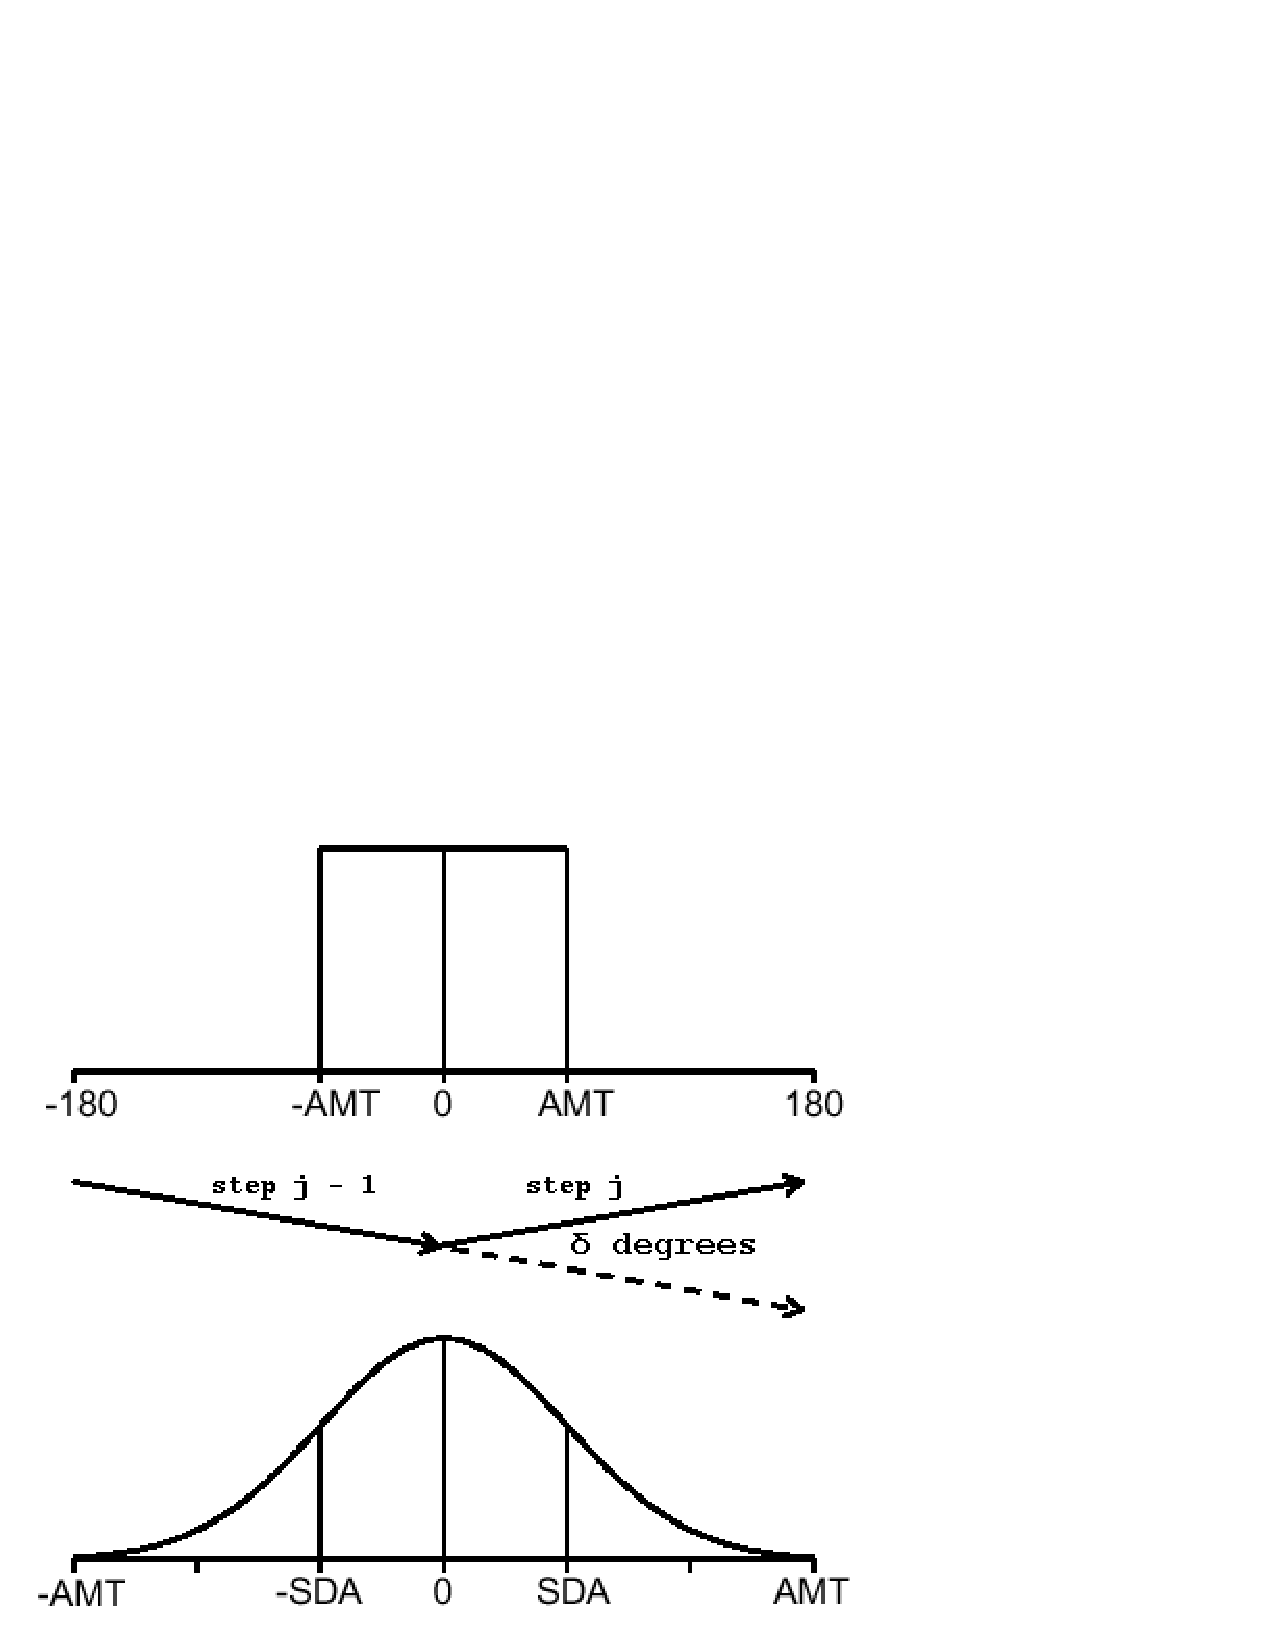
\includegraphics[width=1.0\textwidth]{TADistribution.pdf}
	\end{center}
	\caption{Turning Angle for (a) uniform distribution and (b) depiction
	of what a path may look like.}
\end{figure}
Alternatively, if the animal is already at a plant then the animal picks a random direction uniformly and then takes a step of size $r+1.0$.  This will ensure that the animal will not immediately return to the same plant on the very next step.

\subsection{\emph{Pollination}}
When an animal is on a plant, it collects pollen, distributes pollen, and
consumes food. Each plant contains a number of flowers, $\phi$, from which an
animal may obtain pollen. When an animal visits a plant it picks up pollen from
one or more flowers. The number of flowers from which an animal can obtain
pollen is determined by the total number of flowers on a plant, the fraction of
flowers in bloom at any one time ($a$), the number of times ($j$) the plant has
previously been visited by an animal, and the maximum fraction of flowers
available for pollination ($\eta$). The formula for the number of total flowers
available for visitation during a $k^{th}$ visit to the $j^{th}$ plant
($f_{j,k}$) is given by
\begin{equation}\label{flowers}
	f_{j,k} = \phi \cdot a \cdot \eta^k.
\end{equation}
It is assumed that the amount of food eaten and the amount of pollen collected
is proportional to the number of visited flowers. An animal collects pollen and
eats from every flower that it visits, and so the amount of pollen collected and
the amount of food eaten is proportional to the equation (\ref{flowers}). Let
$f^{\left(i\right)}_{j,k}$ be the number of flowers visited by the $i^{th}$
animal during the $k^{th}$ visit to the $j^{th}$ plant then the amount of
polllen/nectar in the $i^{th}$ animal's stomach after $m$ plant visits is given
by
\[
	c^{\left(i\right)}_m = \sum_{j=0}^{m} \beta f^{\left(i\right)}_{j,k},
\]
where $\beta$ is the proportionallity constant for the amount of pollen
collected at a plant.  Each animal has a maximum amount of food they will ingest, $c_{max}$, at which time they will stop search for food and return to their lair. %The total amount of food that an animal can eat is limited
%by the stomach size, $c_{max}$.

The fraction, $\alpha$, of all flowers are pollinated, and the associated probability that a flower is pollinated, $\rho$, are related by the equation,
\begin{equation} \label{Prob}
	\alpha = \rho \cdot \hat{f}_k.
\end{equation}
Using equation (\ref{limit}) and (\ref{Prob}) we can determine the probability
that a flower is pollinated, $\rho$, by the formula
\[
	\rho = \frac{\alpha}{\phi} \cdot \frac{1 - \eta}{a \cdot \eta}.
\]

When a flower is pollinated it must determined
which previous plant donated the pollen. Each flower visited is
recorded and is available to pollinate the current flower, except those flowers
that are on the same plant. Self- pollination, is not considered, because the
likelyhood of self-pollination is low due to mechanisms that impedes
self-pollination. Each flower considered has an equal likelihood of pollinating
the current flower.

\subsection{Time and Stopping Criteria}
The velocity an animal travels ($v$) is assumed to be constant, as well as the time spent on a plant
($t_{plant}$).  The travel time for an animal is then given by the
formula
\[
	t^{\left(i\right)} = \frac{s^{\left(i\right)}}{v} + T^{\left(i\right)}
\cdot t_{plant},
\]
where $T^{\left(i\right)}$ is the number of plants visited by the $i^{th}$
animal. If we let the maximum allowable travel time be $t_{max}$, then once
$t^{\left(i\right)} \geq t_{max}$ or $c^{\left(i\right)}_m \geq c_{max}$ the
animal is removed from the simulation. $t_{max}$ is based on the optimal searching time during the day.  When there are no animals left the simulation terminates.

\subsection{Model Statistics}
To best explore the inherent differences between biotic and abiotic pollination this study focuses on the effects of movement as well as the effects of plant density.  
\begin{table}[h]\label{eqn}
\begin{tabular}{|l|l|}
  \hline
  % after \\: \hline or \cline{col1-col2} \cline{col3-col4} ...
  Measure & Equation \\ \hline   \hline
  Average Path Distance & $\displaystyle\bar{s} = \frac{1}{b} \sum_{i=1}^b \sum_{j=1}^n s^{\left(i\right)}_j$ \\ \hline
  Average Maximum Distance & $\displaystyle \bar{M} = \frac{1}{b} \sum_{i=1}^b \max_j \sqrt{\left(x^{\left(i\right)}_{1,0}
- x^{\left(i\right)}_{1,j}\right)^2 +
			\left(x^{\left(i\right)}_{2,0} -
x^{\left(i\right)}_{2,j}\right)^2}  $ \\  \hline
  Average Pollination Distance & $\displaystyle \bar{p} = \frac{1}{n} \sum_{i=1}^{n} \left(
\frac{1}{\tau^{\left(i\right)}} \sum_{j=1}^{\tau^{\left(i\right)}}
\sqrt{\left(x^{\left(i\right)}_1 -
x^{\left(j\right)}_1\right)^2 + \left(x^{\left(i\right)}_2 -
		x^{\left(j\right)}_2\right)^2}
		\right)  $ \\  \hline
  Average Maximum Pollination Distance & $\displaystyle \bar{P} = \frac{1}{n} \sum_{i=1}^{n} \max_j \sqrt{\left(x^{\left(i\right)}_1 -
x^{\left(j\right)}_1\right)^2 + \left(x^{\left(i\right)}_2 -
		x^{\left(j\right)}_2\right)^2}$ \\  \hline
  Average Weighted Diversity of Fathers & $\displaystyle E = \frac{1}{n} \sum_{i=1}^n 1/\frac{1}{\left(\tau^{\left(i\right)}\right)^2}
\sum_{j=1}^{\Delta\tau^{\left(i\right)}} F^2_{j,i} $ \\
  \hline
\end{tabular}
\caption{Equations}
\end{table}
In order to quantify these differences we measure statistics that are inherent of the animals: \emph{Average Path Distance}, \emph{Average Maximum Distance}, and those of the plant: \emph{Average Pollination Distance},
\emph{Average Maximum Pollination Distance}, \emph{Average Weighted Diversity of Fathers}.  The calculations of these statistics are given in the Table \ref{eqn}.

In these equations it is assumed that $b$ is the total number of animals, $n$ is the total number of plants, $(x_{1,0}^{(i)},x_{2,0}^{(i)})$ is the starting location of the $i^{th}$ animal, $(x_{1,j}^{(i)},x_{2,j}^{(i)})$ is the location of the $i^{th}$ animal after $j$ steps, $\tau^{(i)}$ is the total number of seeds for the $i^{th}$ plant, $\Delta\tau^{(i)}$ is the number of different fathers contributing pollen to the $i^{th}$ plant, and $F_{j,i}$ is the number of times the $j^{th}$ father contributed pollen to the $i^{th}$ plant.



% -----------------------------------------------------------
\section{{\bf Results}}
The following results are based on simulations of the model with parameter values given in Table \ref{parameter}.  These parameters are based on field data estimates from the VCU Rice Center (unpublished).  The grid size was 101 patches by 101 patches.
\begin{table}
\begin{tabular}{|l|l|l|l|}
  \hline
  % after \\: \hline or \cline{col1-col2} \cline{col3-col4} ...
  Parameter Description & Symbol & Value &  \\ \hline  \label{parameter}
  Total number of animals & b & 1,000 & fixed  \\ \hline
  Maximum time & $t_{max}$ & 1,200 seconds & fixed \\ \hline
  Fraction of blooms at one time & a & 0.2 & fixed \\ \hline
  Maximum fraction of available flowers & $\eta$ & 0.75 & fixed \\ \hline
  Search radius & r & 1.0 & fixed \\ \hline
  Number of flowers per plant & $\phi$ & 100 & fixed \\ \hline
  Probability of pollination   & $\rho$ & 0.4286 & calculated \\ \hline
  Number of plants & n & 1000 & fixed \\ \hline
  Time spent at each plant & $t_{plant}$ & 100 seconds & fixed \\ \hline
\end{tabular}
\caption{Parameter Values}
\end{table}

The standard error was calculated by dividing the sample standard deviation
 by the square root of the total number of samples.   The standard errors were all less than
1\% on average, so will not be shown due to the small size.


Determining the distance animals travel during a foraging trip is important factor for their survivability.  In order for an animal to survive it must find enough food foraging without losing too much energy.  In this study the density of plants is varied, which can directly affect the amount of foraging the animals will be able to achieve in a set amount of time.  The higher the density the greater the potential for the animal to forage.  The maximum angle is also varied.  The relationship of this angle with respect to foraging is a more complicated one.  In terms of foraging, a very small maximum turning angle may not result in successful foraging due to the paths are too linear.  On the other hand, a maximum turning angle which is too large can result in searching patterns that repetitively cover the same area over and over again.

%{\emph{Average Path Distance}}
\begin{figure}
  \begin{center}
  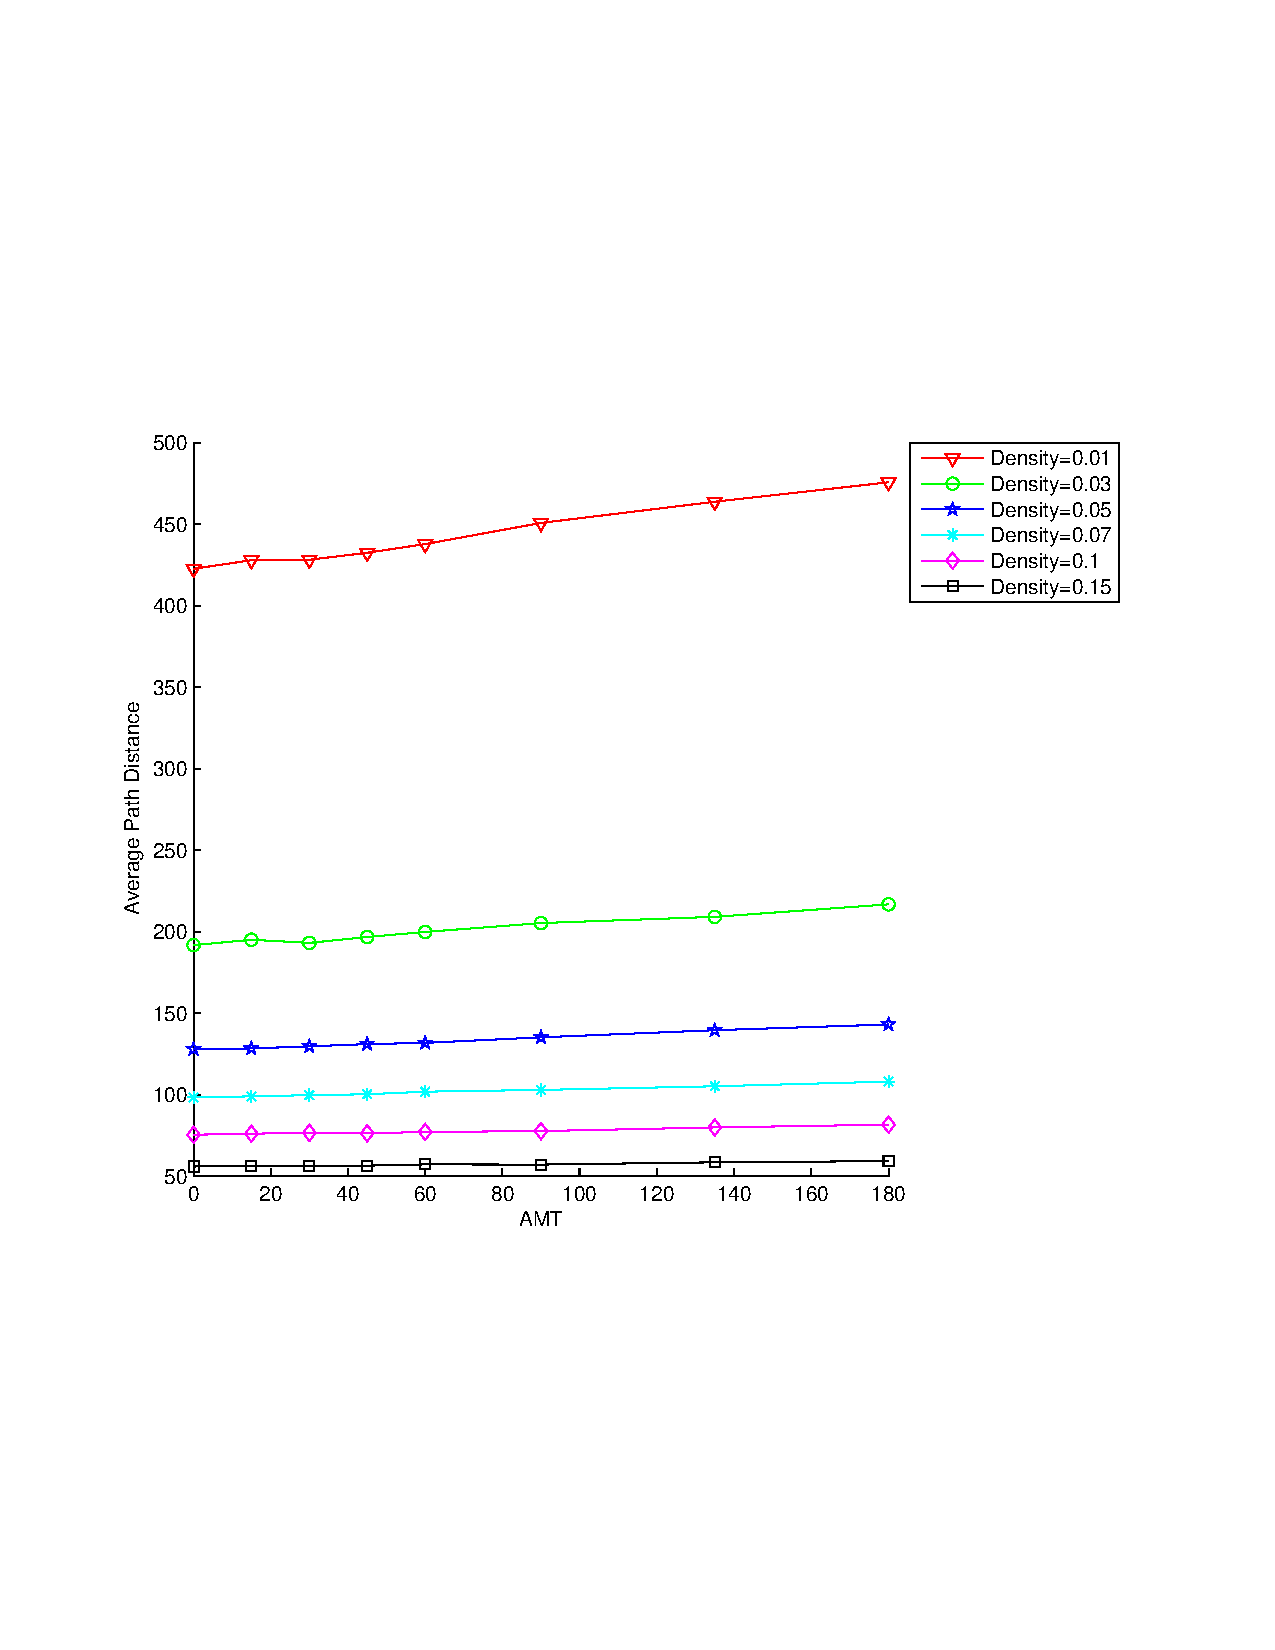
\includegraphics[width=.5\linewidth,scale=.5]{PathVsAMT.pdf}
  \end{center}
  \caption{\small Average Path Distance vs. Turning Angle for Various Plant
Densities}
  \label{AvgPathN}
\end{figure}


In Figure \ref{AvgPathN} the average distance traveled for each animal decreases with increasing density due to higher foraging success.  In this situation the animals will spend more time on plants since they can find plants more readily.  The maximum turning angle does not have a large effect on on the distance.  There is a modest effect of maximum turning angle on low plant density where the larger the angle increases the average distance due to less success of foraging.



The average maximum distance traveled by animals, see Figure \ref{AvgMaxDBees},
is affected by both the turning angle and plant density. As with the average path distance, the maximum distance decreases with higher density which decreases the overall travel time for the animals.  Though in this case due to the movement patterns the angle has a large effect on maximum distance especially at lower densities.  As the maximum angle decreases the animals are more likely to travel directly away from their starting points increasing the maximum distance traveled.

%\subsubsection*{\emph{Average Maximum Distance}}
\begin{figure}
  \begin{center}
  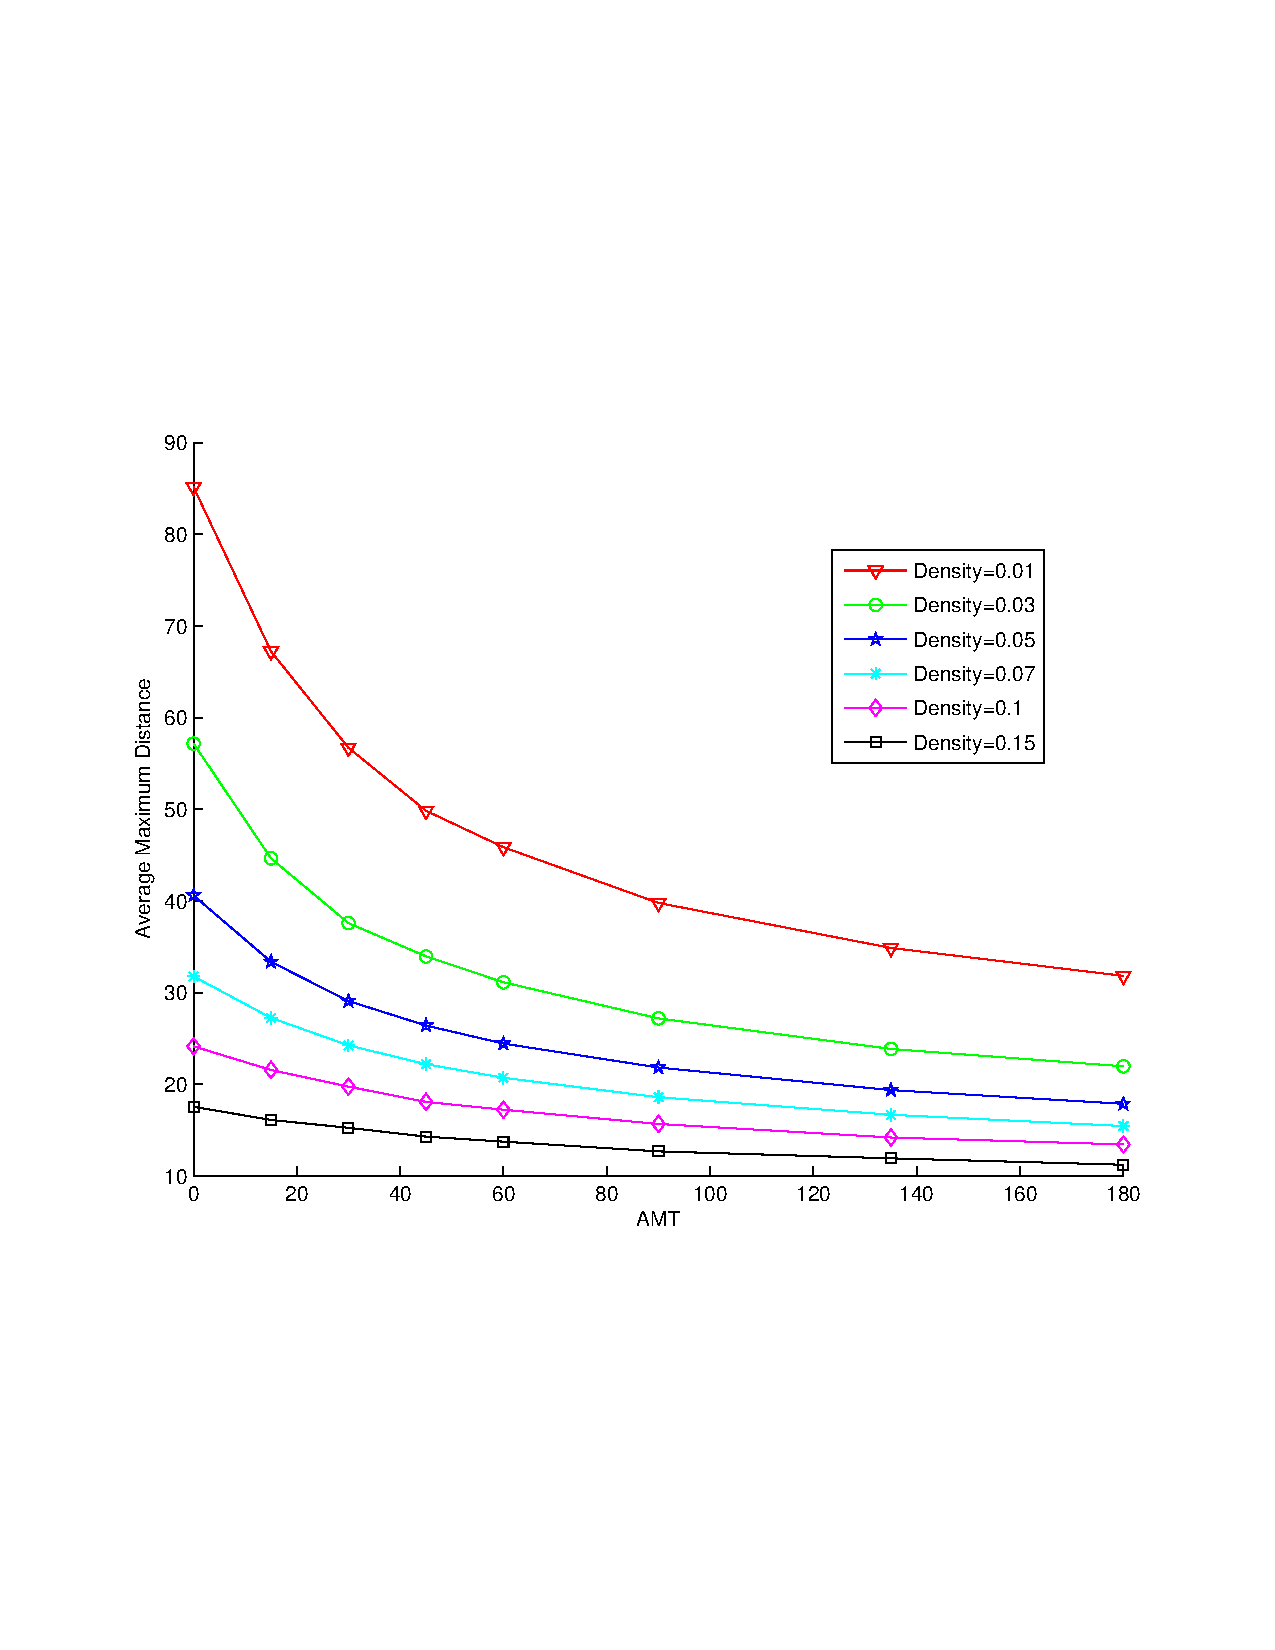
\includegraphics[width=1.0\textwidth]{MaxDVsAMT.pdf}
  \end{center}
  \caption{\small Average Maximum Distance vs. Turning Angle for Various Plant
Densities}
  \label{AvgMaxDBees}
\end{figure}

For a plant density of 0.01 and AMT = $0^\circ$ the average maximum distance is
quadruple of the average maximum distance for a plant density of 0.01 and AMT =
$180^\circ$. For a higher plant density of 0.15 the average maximum distance is
50\% larger. Thus, a purely random diffusion process results in shorter average
maximum distances as compared to smaller turning angles, and as was seen with
the average pollination distance the effect of turning angle is more pronounced
for smaller plant densities. Again, this is expected since for higher plant
densities the animal direction is reset more often and therefore the animal path
becomes more and more like a purely random walk.

%\subsubsection*{\emph{Average Pollination Distance}}
\begin{figure}
  \begin{center}
  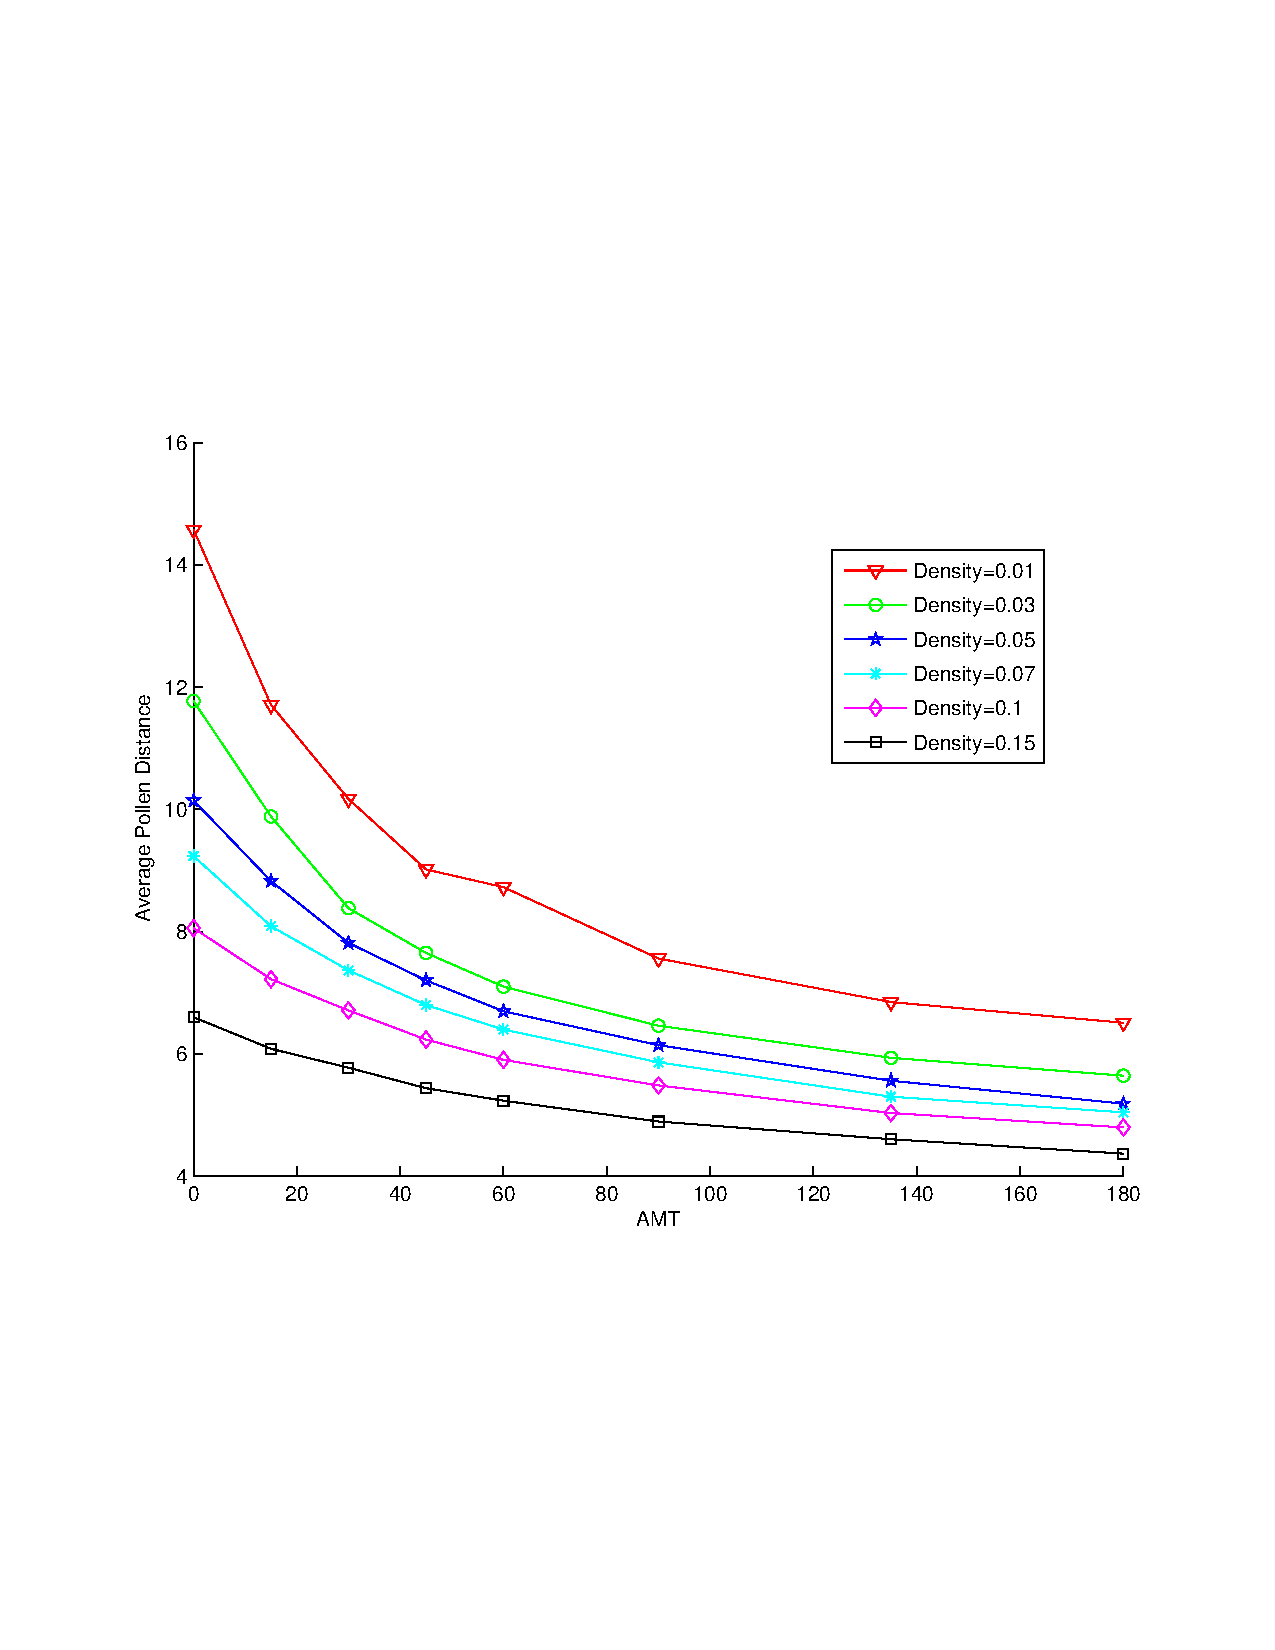
\includegraphics[width=1.0\textwidth]{PollenDVsAMT.pdf}
  \end{center}
  \caption{\small Average Pollination Distance vs. Turning Angle for Various
Plant Densities}
  \label{AvgDist}
\end{figure}

The average pollination distance, see Figure \ref{AvgDist}, decreases with increasing density due to the greater likelihood of pollinating nearby trees.  As with the average maximum distance, as the maximum angle decreases the animal is likely to travel farther from its initial position which allows for longer pollination distances.

For a plant density of 0.01 and AMT = $0^\circ$ the average maximum pollination
distance is approximately triple of that for the same plant density and AMT =
$0^\circ$. Additionally, for plant density of 0.15 and AMT = $0^\circ$ the
average pollination distance is approximately double of the average pollination
distance for the same density and AMT = $180^\circ$. Clearly, the average
pollination distance for wind dispersal is less than that of an average
pollination distance for an animal that follows a straighter path for any of the simulated plant densities.



%\subsubsection*{\emph{Average Maximum Pollination Distance}}
\begin{figure}
  \begin{center}
  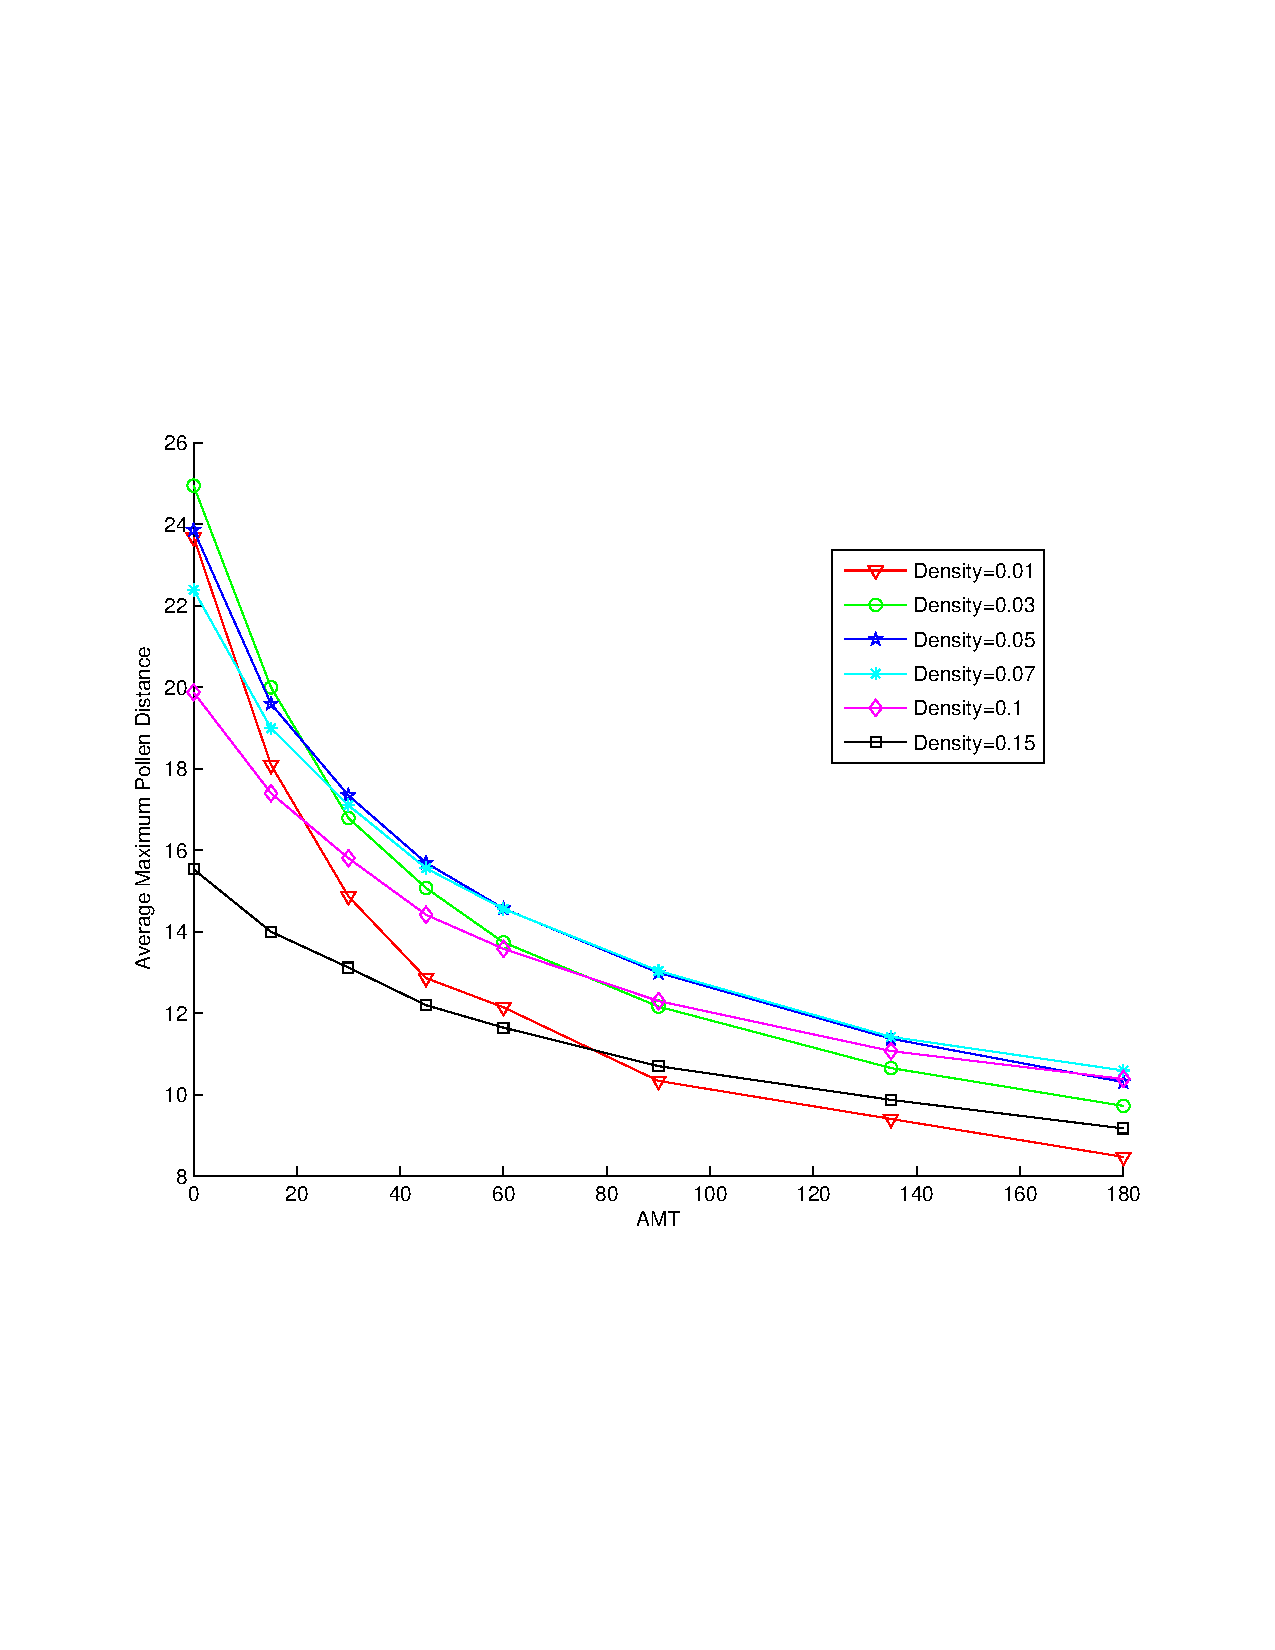
\includegraphics[width=1.0\textwidth]{MaxPollenVsAMT.pdf}
  \end{center}
  \caption{\small Average Maximum Pollination Distance vs. Turning Angle for
Various Plant Densities}
  \label{AvgMaxDTreesN}
\end{figure}

The average maximum pollination distance has a much more complicated relationship with density and maximum turning angle, see Figure \ref{AvgMaxDTreesN}.  
The average maximum pollination distance decreases as maximum turning angle increases from
$0^{\circ}$ to $180^{\circ}$ across all densities. This is due to animals
covering a shorter distance for higher turning angles, and therefore the plants
that are visited will be closer together on average. 

Additionally, we see that
the resultant average maximum pollination distance for a purely random diffusion
process is marketably lower than those for correlated random walks resulting in
straighter animal paths. Thus, wind dispersal will result in an average maximum
pollination distance that is less than the average maximum pollination distance
for a correlated random walk. Thus, one might expect that wind dispersal of
pollen results in a smaller areal extent of gene flow as compared to animal
mediated gene flow.

The density affects the maximum pollination distance in a more complex fashion.  The higher the density the more gradual the decrease is in the maximum pollination distance as the maximum turning angle increases.  Whereas for lower densities this decrease is much larger.  This is likely due to the fact that at lower densities pollination occurs less frequently with a larger variability of maximum pollination distances.

%\subsubsection*{\emph{Average Weighted Diversity of Fathers}}
\begin{figure}
  \begin{center}
  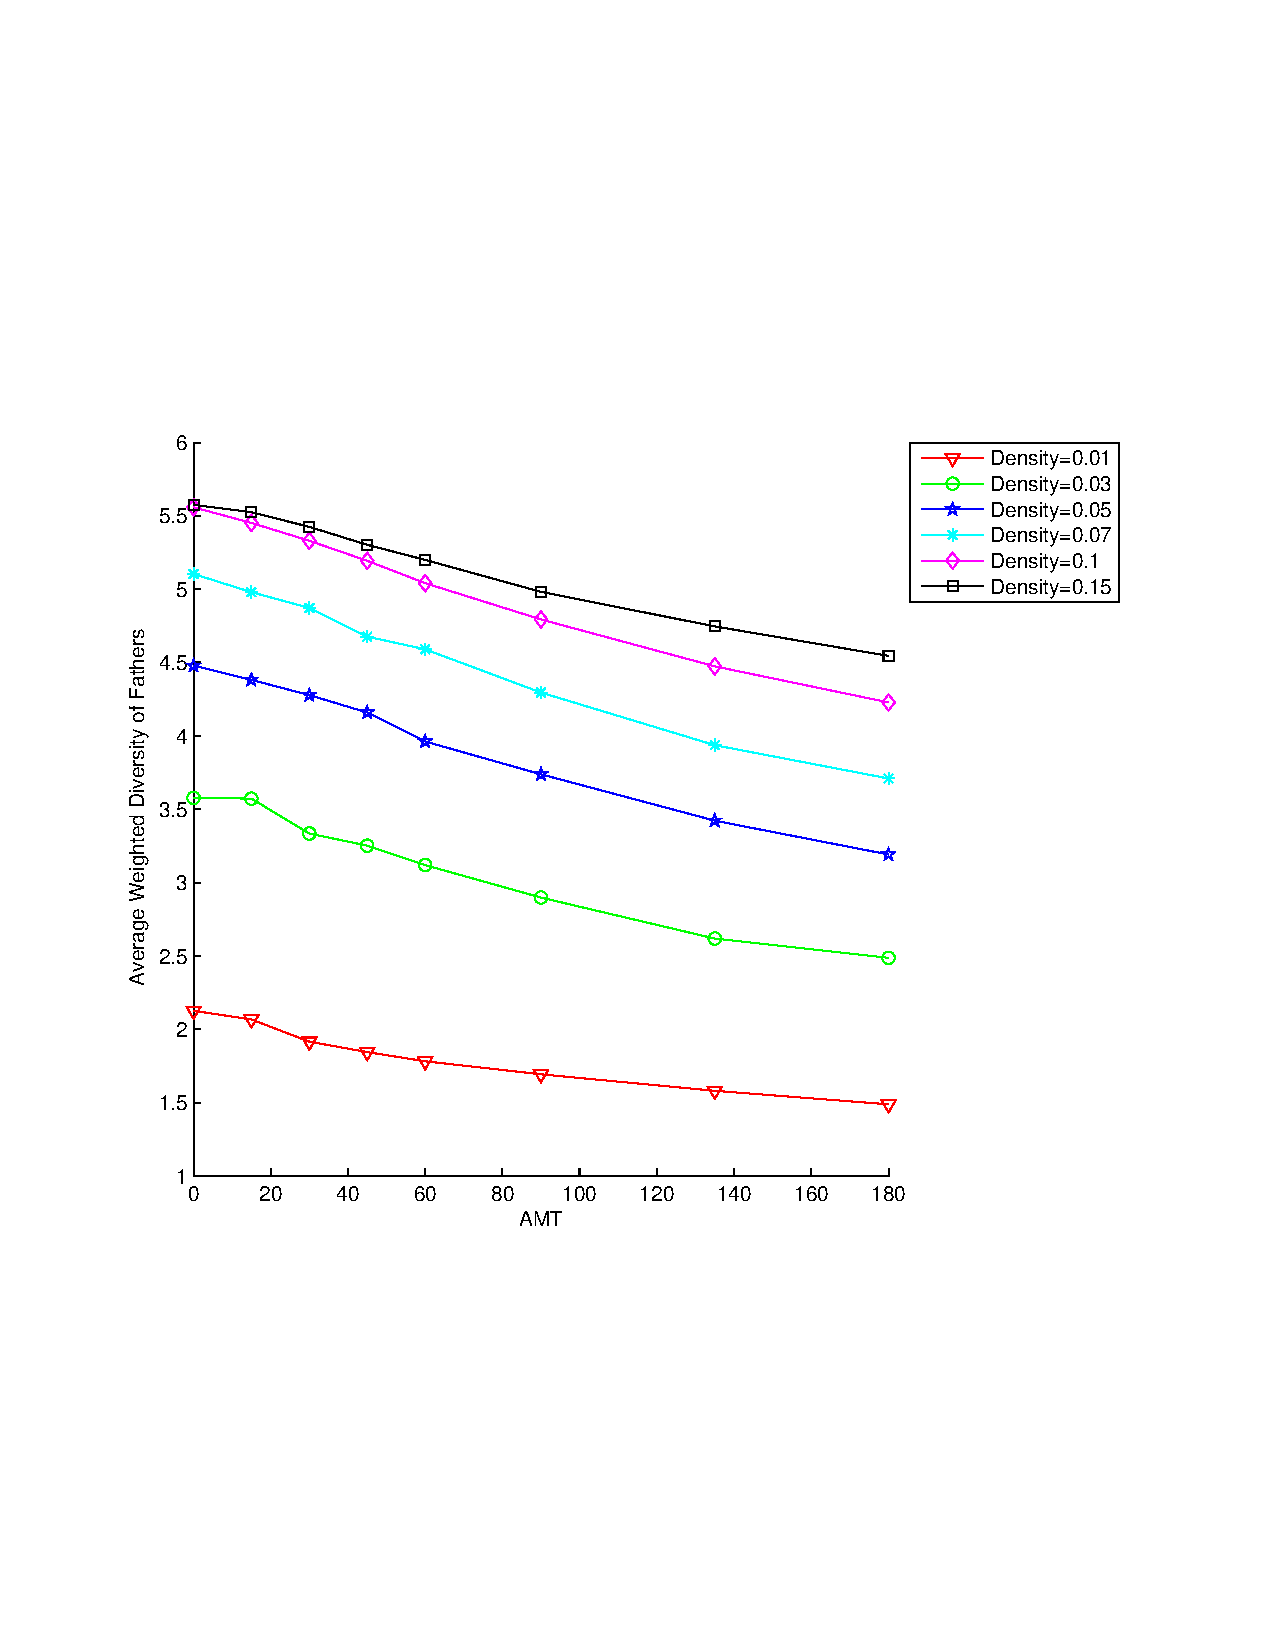
\includegraphics[width=1.0\textwidth]{WDFvsAMT.pdf}
%  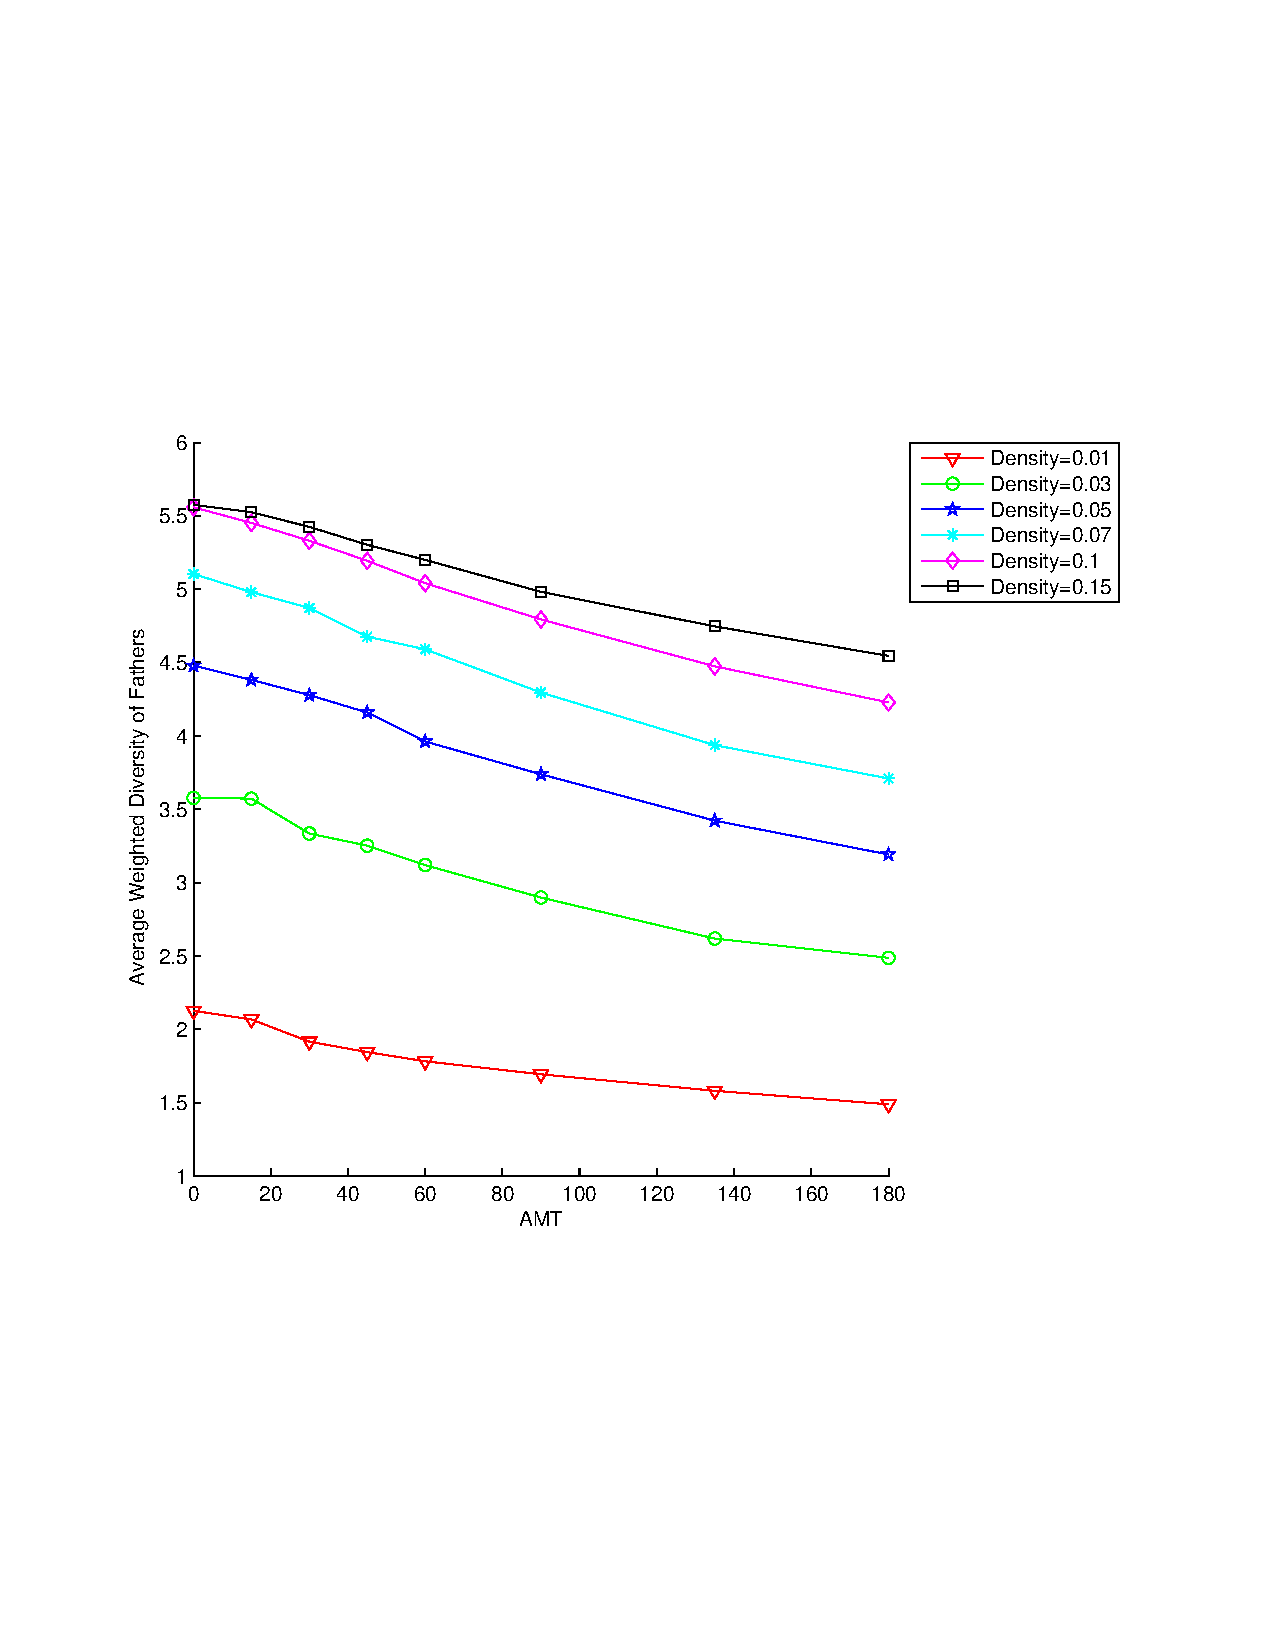
\includegraphics[width=1.0\textwidth,height=0.5\textheight]{WDFvsAMT.pdf}
  \end{center}
  \caption{\small Average Weighted Diversity of Fathers vs. Turning Angle for
Various Plant Densities}
  \label{EFathers}
\end{figure}

In general there is a small decrease in the average weighted diversity of fathers as the maximum turning angle increases, see Figure \ref{EFathers}. With higher maximum turning angles the search patterns tend to be more circular lowering the overall diversity that a plant will see.  On the other hand, by increasing the density, plants will see an increase in diversity due to the larger amount of plants near by.  This increase is lessens at higher densities due to the limited foraging time of the pollinators.



\section{{\bf Discussion}}
There are many factors that affect the dispersal of gene within a species across a landscape.  Each factor may have a large effect on particular statistics such as the average or the maximum pollination distance.  Each of these statistics as well as the actual factors are difficult if not impossible to accurately measure in the field.  The simulations studied here provide insight to the effects of plant density as well as a reasonable model for pollinator movement across the landscape.

The majority of models studying pollination have assumed a purely random
diffusion process. There is clear evidence that there are differences in statistics seen between plants pollinated through wind dispersal from those pollinated through animal dispersal, see ***.
It is demonstrated here through an agent based correlated random walk that if an animal is not moving in a purely random fashion, then important pollination statistics can be dramatically affected. 

As can be seen in the results section the magnitude of turning angle had varying
degrees of effects over different plant densities and therefore pollination
patterns predicted by a model assuming a purely random walk could be vastly
different from a model assuming a correlated random walk. For high plant
densities, the effects of correlated random walk was less pronounced than that of
low plant densities, except for the \emph{average weighted diversity of
fathers}. In the case of \emph{average weighted diversity of fathers} the affect
of turning angle magnitudes were more pronounced for high densities. Therefore,
although diffusion models for densely populated plant species may not vary
greatly from models that assume a correlated random walk for \emph{average
pollination distance} or \emph{average maximum pollination distance} they will
vary significantly for \emph{average weighted diversity of fathers}. This has
the affect of under estimating the diversity of pollination for high plant
densities and animal dispersal as compared to similar plant densities and wind
dispersal.

The variation between correlated random walk and that of a purely random walk is
significant at low plant densities for the statistics such as \emph{average
maximum distance}, \emph{average pollination distance}, and \emph{average
maximum pollination distance} and so for the case of low plant densities the
assumption of a purely random walk may lend to bias in the analysis of
pollination. Most studies to date have been conducted on small herbaceous plant
species whose densities tend to be high. Even though most of the animals
statistics presented were not greatly affected by turning angle for high plant
densities the average weighted diversity of fathers had was still greatly
affected by the turning angle at these densities, and therefore an assumption of
a purely random walk would be an inappropriate assumption and at any of the
densities examined in this study. Therefore a correlated random walk may be a
better approximation to animal movement.

\subsection*{Acknowledgment}


% -----------------------------------------------------------
\bibliographystyle{amsplain}
\bibliography{xbib}
\end{document}
% -----------------------------------------------------------
